\documentclass[fleqn]{article}
\oddsidemargin 0.0in
\textwidth 6.0in
\thispagestyle{empty}
\usepackage{import}
\usepackage{amsmath}
\usepackage{graphicx}
\usepackage{flexisym}
\usepackage{calligra}
\usepackage{amssymb}
\usepackage{bigints} 
\usepackage[english]{babel}
\usepackage[utf8x]{inputenc}
\usepackage{float}
\usepackage[colorinlistoftodos]{todonotes}


\DeclareMathAlphabet{\mathcalligra}{T1}{calligra}{m}{n}
\DeclareFontShape{T1}{calligra}{m}{n}{<->s*[2.2]callig15}{}
\newcommand{\scriptr}{\mathcalligra{r}\,}
\newcommand{\boldscriptr}{\pmb{\mathcalligra{r}}\,}

\definecolor{hwColor}{HTML}{442020}

\begin{document}

  \begin{titlepage}

    \newcommand{\HRule}{\rule{\linewidth}{0.5mm}}

    \center

    \begin{center}
      
\includegraphics[height=11cm, width=11cm]{asu.png}
    \end{center}

    \vline

    \textsc{\LARGE Classical Parts/Field/Matter III}\\[1.5cm]

    \HRule \\[0.5cm]
    { \huge \bfseries Homework 9}\\[0.4cm] 
    \HRule \\[1.0cm]

    \textbf{Behnam Amiri}

    \bigbreak

    \textbf{Prof: Samuel Teitelbaum}

    \bigbreak

    \textbf{{\large \today}\\[2cm]}

    \vfill

  \end{titlepage}

  \begin{enumerate}
    \item \textbf{11.14 (30 points)} In Bohr's theory of hydrogen, the electron in its ground state was
    supposed to travel in a circle of radius $5 \times 10^{-11} ~ m$, held in orbit by the Coulomb
    attraction of the proton. According to classical electrodynamics, this electron should
    radiate, and hence spiral in to the nucleus. Show that $v<<c$ for most of the trip
    (so you can use the Larmor formula), and calculate the lifespan of Bohr's atom.
    (Assume each revolution is essentially circular.)

        \textcolor{hwColor}{
          \\
          We know that centripetal force is a force that makes a body follow a curved path. Its direction is 
          always orthogonal to the motion of the body and towards the fixed point of the instantaneous 
          center of curvature of the path. And it is mathematical formula is $F_c=\dfrac{m v^2}{r}$. 
          In chapter 2 we were introduced with the Coulomb's law 
          $(F=\dfrac{1}{4 \pi \epsilon_0} \dfrac{q Q}{r^2} \hat{\scriptr})$ which is an 
          experimental law of physics that quantifies the amount of force between two stationary, 
          electrically charged particles. Equating the two formulas gives us:
          \\
          \\
          $
            F_c=F \Longrightarrow \dfrac{m v^2}{r}=\dfrac{1}{4 \pi \epsilon_0} \dfrac{q^2}{r^2}
            \\
            \\
            \\
            mv^2=\dfrac{1}{4 \pi \epsilon_0} \dfrac{q^2}{r}
            \Longrightarrow \boxed{
              v=\sqrt{\dfrac{1}{4 \pi \epsilon_0} \dfrac{q^2}{rm}}
            } ~~~~ \checkmark
            \\
            \\
            \\
            \begin{cases}
              \text{Electron mass: } 9.1093837 \times 10^{-31} ~ kg
              \\
              \\
              \text{Radius: } 5 \times 10^{-11} ~ m
              \\
              \\
              \text{Charge: } 1.60217663 \times 10^{-19} ~ C
            \end{cases} \Longrightarrow
            v=\sqrt{\dfrac{1}{4 \pi \epsilon_0} \dfrac{q^2}{rm}}
            =\sqrt{\dfrac{1}{4 \pi \epsilon_0} \dfrac{\bigg( 1.60217663 \times 10^{-19} \bigg)^2}{ \bigg( 5 \times 10^{-11} ~ m \bigg) \times\bigg( 9.1093837 \times 10^{-31} ~ kg \bigg) }}
            \\
            \\
            \\
            \therefore ~~~ \boxed{
              v=2251149.43608 ~ m/s
            }
            \\
            \\
          $
          From page $481$ we have the \textbf{Larmor formula} as $P=\dfrac{\mu_0 q^2 a^2}{6 \pi c}$. Assuming the 
          total energy of electron as $U$:
          \\
          \\
          \\
          $
            \begin{cases}
              F=ma=\dfrac{mv^2}{r}
              \\
              \\
              P=\dfrac{\mu_0 q^2 a^2}{6 \pi c}
            \end{cases} \Longrightarrow P=\dfrac{\mu_0 q^2}{6 \pi c} \bigg( \dfrac{v^2}{r} \bigg)^2
            =\dfrac{\mu_0 q^2}{6 \pi c} \left[\dfrac{\bigg( \sqrt{\dfrac{1}{4 \pi \epsilon_0} \dfrac{q^2}{rm}} \bigg)^2}{r} \right]^2
            =\dfrac{\mu_0 q^2}{6 \pi c} \bigg( \dfrac{1}{4 \pi \epsilon_0} \dfrac{q^2}{r^2 m} \bigg)^2 ~~~~~ (A)
            \\
            \\
            \\
            U=P.E.+K.E.=-\dfrac{1}{4 \pi \epsilon_0} \dfrac{q^2}{r}+\dfrac{1}{2} m v^2
            =-\dfrac{1}{4 \pi \epsilon_0} \dfrac{q^2}{r}+\dfrac{1}{2} m \left[\sqrt{\dfrac{1}{4 \pi \epsilon_0} \dfrac{q^2}{rm}}\right]^2
            \\
            \\
            =-\dfrac{1}{4 \pi \epsilon_0} \dfrac{q^2}{r}+\dfrac{1}{2} m \dfrac{1}{4 \pi \epsilon_0} \dfrac{q^2}{rm}
            \Longrightarrow \boxed{U=-\dfrac{1}{8 \pi \epsilon_0}\dfrac{q^2}{r}} 
            \\
            \\
            \\
            P=-\dfrac{dU}{dt}=-\dfrac{d}{dt} \left[-\dfrac{1}{8 \pi \epsilon_0} \dfrac{q^2}{r}\right]
            =\dfrac{q^2}{8 \pi \epsilon_0} \dfrac{dr}{dt}
            \\
            \\
            \\
            \therefore ~~~ \boxed{
              P=-\dfrac{1}{8 \pi \epsilon_0} \dfrac{q^2}{r^2} \dfrac{dr}{dt}
            } ~~~~~ (B)
            \\
            \\
            \\
            \begin{cases}
              \text{From (A): } P=\dfrac{\mu_0 q^2}{6 \pi c} \bigg( \dfrac{1}{4 \pi \epsilon_0} \dfrac{q^2}{r^2 m} \bigg)^2
              \\
              \\
              \text{From (B): } P=-\dfrac{1}{8 \pi \epsilon_0} \dfrac{q^2}{r^2}
            \end{cases}
            \Longrightarrow
            \dfrac{\mu_0 q^2}{6 \pi c} \bigg( \dfrac{1}{4 \pi \epsilon_0} \dfrac{q^2}{r^2 m} \bigg)^2
            =-\dfrac{1}{8 \pi \epsilon_0} \dfrac{q^2}{r^2} \dfrac{dr}{dt}
            \\
            \\
            \\
            dt=-dr ~ 3c r^2 \bigg( \dfrac{2 \pi \epsilon_0 m c}{q^2} \bigg)^2
            \\
            \\
            \\
            t=\bigints dt=\bigints\limits_{r_A}^{0} -dr ~ 3c r^2 \bigg( \dfrac{2 \pi \epsilon_0 m c}{q^2} \bigg)^2
            \\
            \\
            \\
            \therefore ~~~ \boxed{
              t=r^3_A ~ c \bigg( \dfrac{2 \pi \epsilon_0 mc}{q^2} \bigg)^2
            } ~~~~ \checkmark
            \\
            \\
            \text{Plugging in the vales we have gives us:}
            \\
            \\
            t=\bigg( 5 \times 10^{-11} \bigg)^3 ~  \bigg( 3 \times 10^8 \bigg) 
            \bigg( \dfrac{
              2 \pi \bigg( 8.85 \times 10^{-12} \bigg) \bigg( 9.1093837 \times 10^{-31} \bigg) \bigg( 3 \times 10^8  \bigg)
            }{
              \bigg( 1.60217663 \times 10^{-19} \bigg)^2
            } \bigg)^2
            \\
            \\
            \\
            \therefore ~~~ \boxed{
              t \approxeq 1.3141 \times 10^{-11} ~ s
            }
          $
        }

    \pagebreak

    \item \textbf{11.17 (30 points)} 
    \begin{enumerate}
      \item A particle of charge $q$ moves in a circle of radius $R$ at a constant speed $v$. To sustain the motion, 
      you must, of course, provide a centripetal force $m v^2/R$; what additional force $(F_e)$ must you exert, 
      in order to counteract the radiation reaction? [It's easiest to express the answer in terms of the instantaneous
      velocity $v$.] What power $(P_e)$ does this extra force deliver? Compare $P_e$ with the
      power radiated (use the Larmor formula).

      \item Repeat part $(a)$ for a particle in simple harmonic motion with amplitude $A$ and
      angular frequency $\omega: w(t) = A cos(\omega t) \hat{z}$. Explain the discrepancy.


      \item Consider the case of a particle in free fall (constant acceleration g). What is
      the radiation reaction force? What is the power radiated? Comment on these
      results.

    \end{enumerate}
    
    \begin{center}
      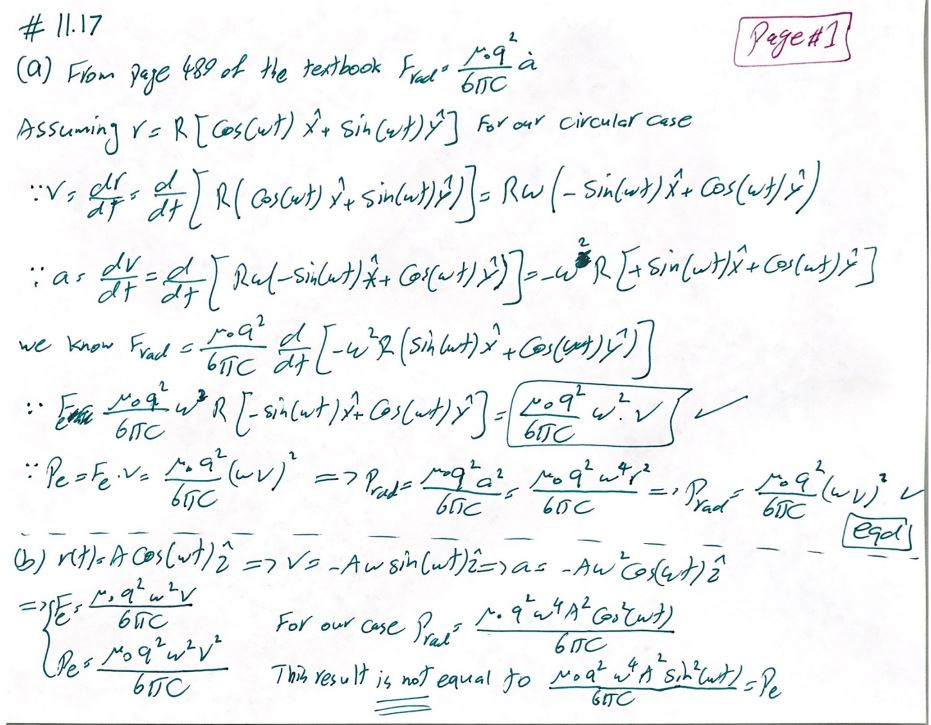
\includegraphics[height=13cm, width=15cm]{1117A.JPG}
    \end{center}

    \pagebreak

    \begin{center}
      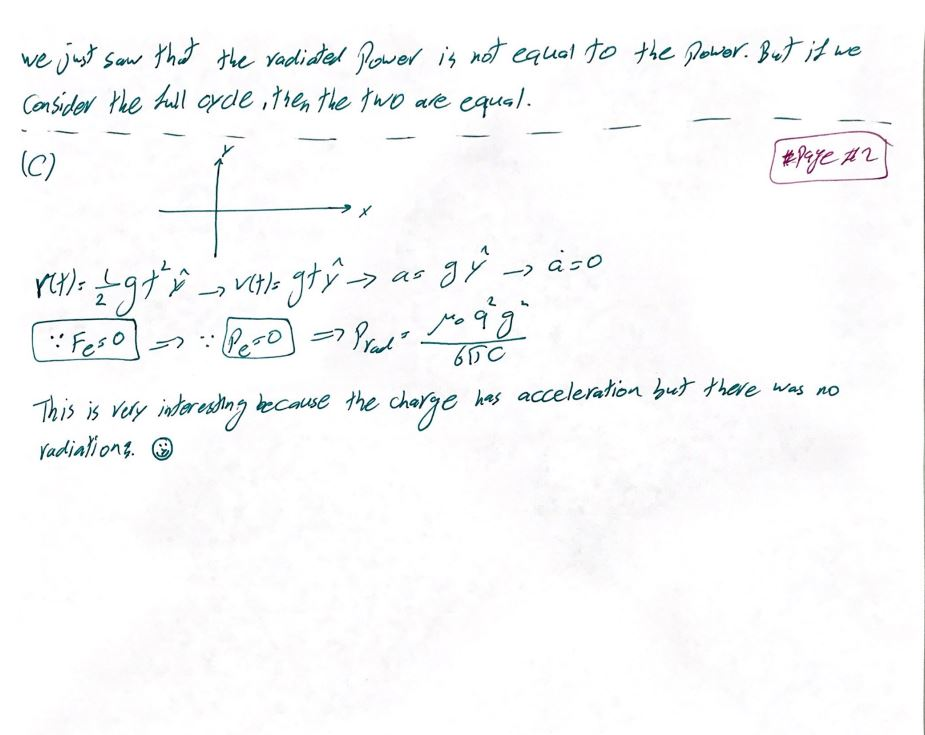
\includegraphics[height=13cm, width=15cm]{1117B.JPG}
    \end{center}

    \pagebreak

    \item \textbf{11.18 (40 points)} A point charge $q$, of mass $m$, is attached to a spring of constant $k$.
    At time $t=0$ it is given a kick, so its initial energy is $U_0=\dfrac{1}{2} m v^2_0$. Now it oscillates,
    gradually radiating away this energy.
    \begin{enumerate}
      \item Confirm that the total energy radiated is equal to $U_0$. Assume the radiation
      damping is small, so you can write the equation of motion as
      $$
        \ddot{x}+\gamma \dot{x}+\omega_0 x=0,
      $$
      and the solution as
      $$
        x(t)=\dfrac{v_0}{\omega_0} e^{-\gamma t/2} sin(\omega_0 t),
      $$
      with $\omega_0 \equiv \sqrt{k/m}, ~ \gamma=\omega_0 \tau,$ and $\gamma << \omega_0$ (drop $\gamma^2$ in comparison 
      to $\omega^2_0$, and when you average over a complete cycle, ignore the change in $e^{-\gamma t}$).


      \item Suppose now we have two such oscillators, and we start them off with identical
      kicks. Regardless of their relative positions and orientations, the total energy
      radiated must be $2 U_0$. But what if they are right on top of each other, so it's
      equivalent to a single oscillator with twice the charge; the Larmor formula says
      that the power radiated is four times as great, suggesting that the total will be
      $4 U_0$. Find the error in this reasoning, and show that the total is actually $2 U_0$, as
      it should be.


    \end{enumerate}

    \begin{center}
      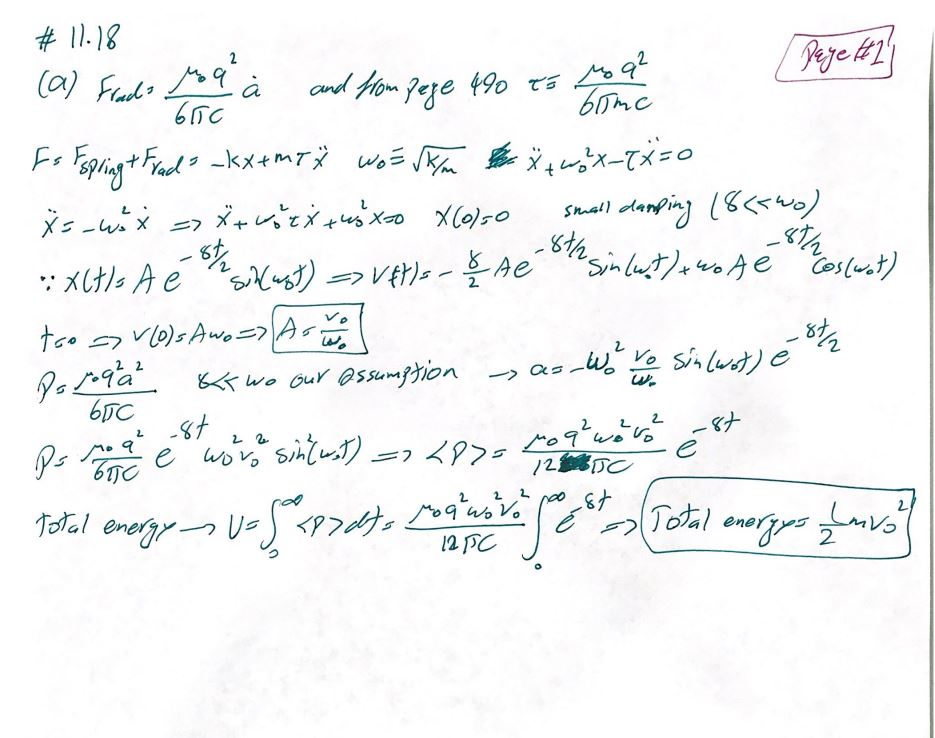
\includegraphics[height=13cm, width=15cm]{1118A.JPG}
    \end{center}

    \pagebreak

    \begin{center}
      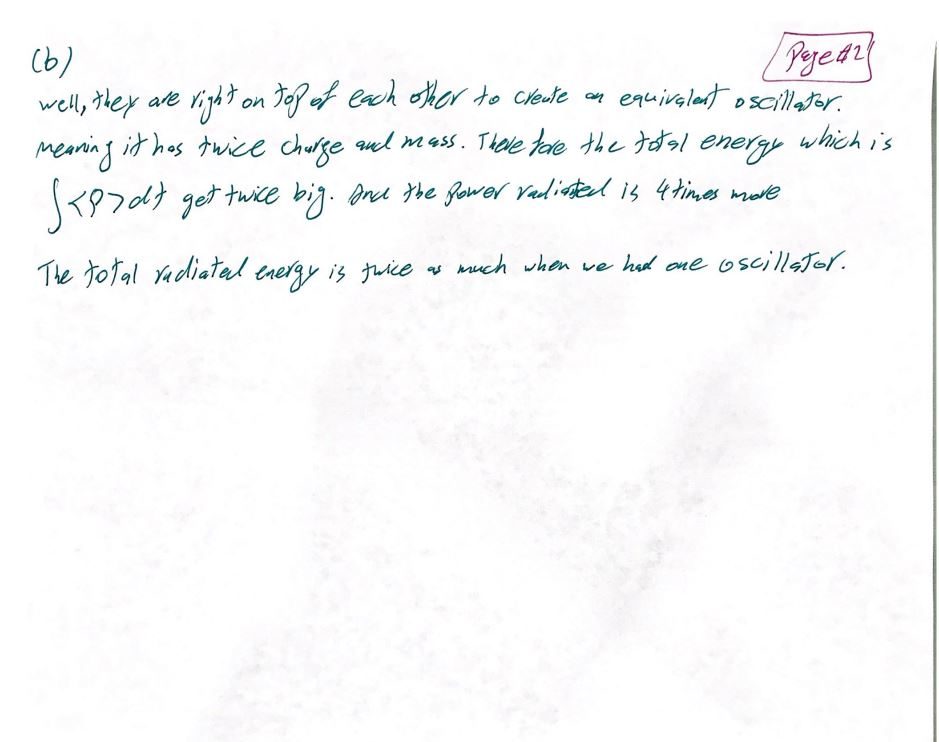
\includegraphics[height=13cm, width=15cm]{1118B.JPG}
    \end{center}

  \end{enumerate}

\end{document}
